% ★★ 中档
\newcommand{\qConicDefThreeSlopeProofStem}{
设 $A, B$ 为椭圆 $C: \frac{x^2}{a^2} + \frac{y^2}{b^2} = 1\ (a>b>0)$ 的长轴两端点，$P$ 是椭圆上异于 $A, B$ 的任意一点．证明：动点 $P$ 与两端点连线的斜率乘积 $k_{PA} \cdot k_{PB}$ 为定值 $-\frac{b^2}{a^2}$，并说明该定值与离心率 $e$ 的关系．
}
\newcommand{\qConicDefThreeSlopeProofFigure}{
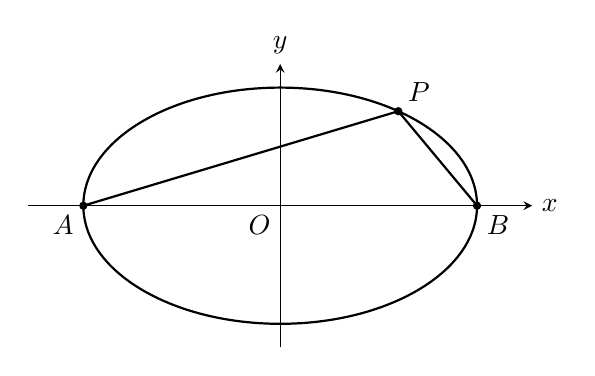
\begin{tikzpicture}[scale=1, >=stealth]
  % Axes
  \draw[->] (-3.2,0) -- (3.2,0) node[right] {$x$};
  \draw[->] (0,-1.8) -- (0,1.8) node[above] {$y$};
  \node[below left] at (0,0) {$O$};
  
  % Ellipse
  \draw[thick] (0,0) ellipse (2.5 and 1.5);
  
  % Endpoints A, B
  \coordinate (A) at (-2.5, 0);
  \coordinate (B) at (2.5, 0);
  \fill (A) circle (1.5pt) node[below left] {$A$};
  \fill (B) circle (1.5pt) node[below right] {$B$};
  
  % Point P
  \coordinate (P) at (1.5, 1.2);
  \fill (P) circle (1.5pt) node[above right] {$P$};
  
  % Lines
  \draw[thick] (P) -- (A);
  \draw[thick] (P) -- (B);
\end{tikzpicture}
}
\newcommand{\qConicDefThreeSlopeProofAnswer}{
证明见解析．斜率积为定值 $-\frac{b^2}{a^2}$，该定值等于 $e^2 - 1$．
}
\newcommand{\qConicDefThreeSlopeProofSolution}{
\begin{proof*}
由题意，椭圆的长轴两端点分别为 $A(-a, 0)$ 和 $B(a, 0)$．\\
设动点 $P(x_0, y_0)$，因为 $P$ 异于 $A, B$，所以 $x_0 \neq \pm a$．\\
根据斜率公式，动点 $P$ 与两端点连线的斜率分别为：
\[
k_{PA} = \frac{y_0 - 0}{x_0 - (-a)} = \frac{y_0}{x_0 + a}
\]
\[
k_{PB} = \frac{y_0 - 0}{x_0 - a} = \frac{y_0}{x_0 - a}
\]
两斜率的乘积为：
\[
k_{PA} \cdot k_{PB} = \frac{y_0}{x_0 + a} \cdot \frac{y_0}{x_0 - a} = \frac{y_0^2}{x_0^2 - a^2}
\]
% ... Rest of proof ...
因为点 $P(x_0, y_0)$ 在椭圆 $\frac{x^2}{a^2} + \frac{y^2}{b^2} = 1$ 上，所以满足：
\[
\frac{x_0^2}{a^2} + \frac{y_0^2}{b^2} = 1 \implies \frac{y_0^2}{b^2} = 1 - \frac{x_0^2}{a^2} = \frac{a^2 - x_0^2}{a^2}
\]
从而得到：
\[
y_0^2 = -\frac{b^2}{a^2} (x_0^2 - a^2)
\]
将 $y_0^2$ 代入斜率乘积公式中得：
\[
k_{PA} \cdot k_{PB} = \frac{-\frac{b^2}{a^2} (x_0^2 - a^2)}{x_0^2 - a^2} = -\frac{b^2}{a^2}
\]
由于 $a, b$ 是常数，故斜率乘积 $k_{PA} \cdot k_{PB}$ 为定值 $-\frac{b^2}{a^2}$．\\
又因为离心率 $e = \frac{c}{a}$，且 $b^2 = a^2 - c^2$，所以：
\[
e^2 - 1 = \frac{c^2}{a^2} - 1 = \frac{c^2 - a^2}{a^2} = -\frac{a^2 - c^2}{a^2} = -\frac{b^2}{a^2}
\]
因此，斜率乘积的定值 $k_{PA} \cdot k_{PB} = e^2 - 1$．
\end{proof*}
}
\newcommand{\qConicDefThreeSlopeProofDiagnosis}{
\errortag{点差法混淆} 部分学生可能尝试直接使用点差法进行证明，但由于 $A, B$ 是长轴端点，且点对称，直接设而不求联立更为直观简洁，点差法容易在此处绕远．\\
\errortag{分母为零讨论缺失} 证明中必须强调 $x_0 \neq \pm a$，否则斜率不存在，公式无意义．
}
